\documentclass[
  12pt, % Fontsize
  a4paper, % papersize
  oneside, % For twosided documents
  openany, 
  numbers=noenddot, % No final dots in Sectionnumbers, e.g 1.2 instead of 1.2.
  BCOR=5mm, % Correction length for lost space from binding
  parskip=half*, %No indent but spacing between paragraphs
  thesis, % type of document
]{bfhbook}


% Test Template for bfhbook.cls
\usepackage[T1]{fontenc}
% Coding 
\usepackage[utf8]{inputenc}
% Language setting
\usepackage[german]{babel}
\usepackage[export]{adjustbox}

% \usepackage{fonttable}
% Hyperref
\usepackage[                
  pdftex,                  % for PDF
  colorlinks=true,         % colored links
  linkcolor=black,         % color for links
  citecolor=black,         % color for references
  urlcolor=black,          % color for url 
  bookmarks=true
]{hyperref}              

\usepackage{booktabs} % For nicer tables
\usepackage{threeparttable} % Table-Captions having the same width than the table
\usepackage[singlelinecheck=off]{caption}
\usepackage{siunitx} % Scientific Units and number setting

\definecolor{codegreen}{rgb}{0,0.6,0}
\definecolor{codegray}{rgb}{0.5,0.5,0.5}
\definecolor{codepurple}{rgb}{0.58,0,0.82}
\definecolor{backcolour}{rgb}{0.95,0.95,0.92}

\usepackage{listings} % For Program-Code
\lstdefinestyle{mystyle}{
    backgroundcolor=\color{backcolour},   
    commentstyle=\color{codegreen},
    keywordstyle=\color{magenta},
    numberstyle=\tiny\color{codegray},
    stringstyle=\color{codepurple},
    basicstyle=\ttfamily\footnotesize,
    breakatwhitespace=false,         
    breaklines=true,                 
    captionpos=b,                    
    keepspaces=true,                 
    numbers=left,                    
    numbersep=5pt,                  
    showspaces=false,                
    showstringspaces=false,
    showtabs=false,                  
    tabsize=2
}
 
\lstset{style=mystyle}

\usepackage{enumitem}
\setlist[description]{style=nextline}

\usepackage{caption}
\captionsetup[figure]{font=footnotesize, labelfont=small}
\newcommand{\source}[1]{\caption*{Quelle: {#1}} }

\usepackage{xcolor}

\usepackage[export]{adjustbox}
\usepackage[document]{ragged2e} % left-alignment for text

\usepackage[acronym]{glossaries}
\makenoidxglossaries

\definecolor{foldercolor}{RGB}{124,166,198}

\usepackage[style=apa]{biblatex}
\addbibresource{references.bib}
\defbibheading{bibliography}[\bibname]{{\section#1}}

% end definition directory tree

%%%%%%%%%%%%%%%%%%%%%%%%%%%%%%%%%%%
% Settings 
%%%%%%%%%%%%%%%%%%%%%%%%%%%%%%%%
% Type?? (Lecture Notes, BSc Thesis, Master Thesis, . . .) 
% Use Variables \BSc, \Master, etc. for language support
\type{Master Thesis}
% Author(s)
\author{Marc Habegger}
% Title
\title{Explainable AI}
% Short Title, will be used in the footline
\shorttitle{MAS Data Science Master Thesis}
% Subtitle
\subtitle{Stand der Forschung und Technik}
% Titlepicture
% \titlepicture{Bilder/Titel.png}
%%

% Topic of Study
\degreeprogramme{MAS Data Science}
% Expert
\expert{Max Kleiner}
% Version
\version{1.0}
% Date
\date{\today} % Or any other possible date

% Departement
% Use Variable for language support
%\TI

% Semester
% Use Variable for language support
%\semester

% Logo(s)

% Colors
% Secondary Color for Graphics, Tables etc.
% Naming: BFH*Color*light|middle|dark, e.g. BFHGreendark, BFHBluelight, etc.
% Possible Color Values: Green, Blue, Purple, Brown 
\newcommand{\seccolor}{BFHLightGreen} 
\newcommand{\imgText}[2]{
\begin{center}
    \begin{minipage}[t]{0.6\textwidth}
    		\vspace{0pt}
		\includegraphics[width=10cm, left]{Bilder/#1}
	\end{minipage}\hfill
    \begin{minipage}[t]{0.4\textwidth}
    		\vspace{0pt}
  		#2
    \end{minipage}
\end{center}
}

\setcounter{secnumdepth}{4}
\setcounter{tocdepth}{4}

% Variablen für diese Arbeit
\newcommand{\compImgSize}{4cm}

% Glossar Einträge
\makeindex

\newglossaryentry{MLg}
{
	name=Machine Learning,
	description={deutsch Maschinelles lernen. Ein künstliches System lernt aus Beispielen und kann diese nach Beendigung der Lernphase verallgemeinern..  \break
	\url{https://de.wikipedia.org/wiki/Maschinelles_Lernen}}
}

\newglossaryentry{ML}{type=\acronymtype, name={ML}, description={Machine Learning}, first={Machine Learning (ML)\glsadd{MLg}}, see=[Glossary:]{MLg}
}

\newacronym{xai}{XAI}{Explainable artificial intelligence}

\newglossaryentry{XAI}
{
	name=Explainable artificial intelligence,
	description={deutsch erklärbare künstliche Inteligenz, Methodiken um Menschen die Vorhersagen durch Modelle des maschinellen Lernens zu erläutern.  \break
	\url{https://en.wikipedia.org/wiki/Explainable_artificial_intelligence}}
}

\newacronym{cnn}{CNN}{Convolutional Neural Network}

\newacronym{dnn}{DNN}{Deep Neural Network}

\newglossaryentry{DNN}
{
    name=Deep Neural Network,
    description={deutsch tiefes lernen, Bezeichnet Neuronale Netze mit vielen Zwischenschichten.\break 
    \url{https://en.wikipedia.org/wiki/Deep_learning\#Deep_neural_networks}}
}

\newacronym{lrp}{LRP}{Layer-wise Relevance Propagation}

\newglossaryentry{LRP}                                 
{
	name=Layer-wise Relevance Propagation,
	description={Technik zur Bestimmung der Merkmale welche am stärksten für das Endresultat verantwortlich sind.}                                   
}                             

\newglossaryentry{Black Box}                                 
{
	name=Black Box,
	description={System welches nicht im Quellcode vorhanden ist und dadurch nicht durch Analyse der Programmierung verstanden werden kann. Jegliche Rückschlüsse sind nur durch Beobachtungen möglich}                                   
}     

\newglossaryentry{DT}                                 
{
	name=Decision Tree,
	description={Entscheidungsbaum, Familie von ML Algorithmen}                                   
}     

\newglossaryentry{Grad CAM}
{
	name=Grad CAM,
	description={Gradient-weighted Class Activation Mapping, Technik welche für eine Entscheidung relevanten Bildinhalte optisch hervorhebt}  
}

\begin{document}
                         
\maketitle
%**************************************************************************
%\frontmatter % preliminary parts

\tableofcontents
\sloppy
%%%%%%%%%%%%%%%%%%%%%%%%
% Introduction
%**************************************************************************
\mainmatter % The main part
%**************************************************************************
%\part{Part One}

\chapter{Einleitung}
\begin{figure}[ht]
\centering
	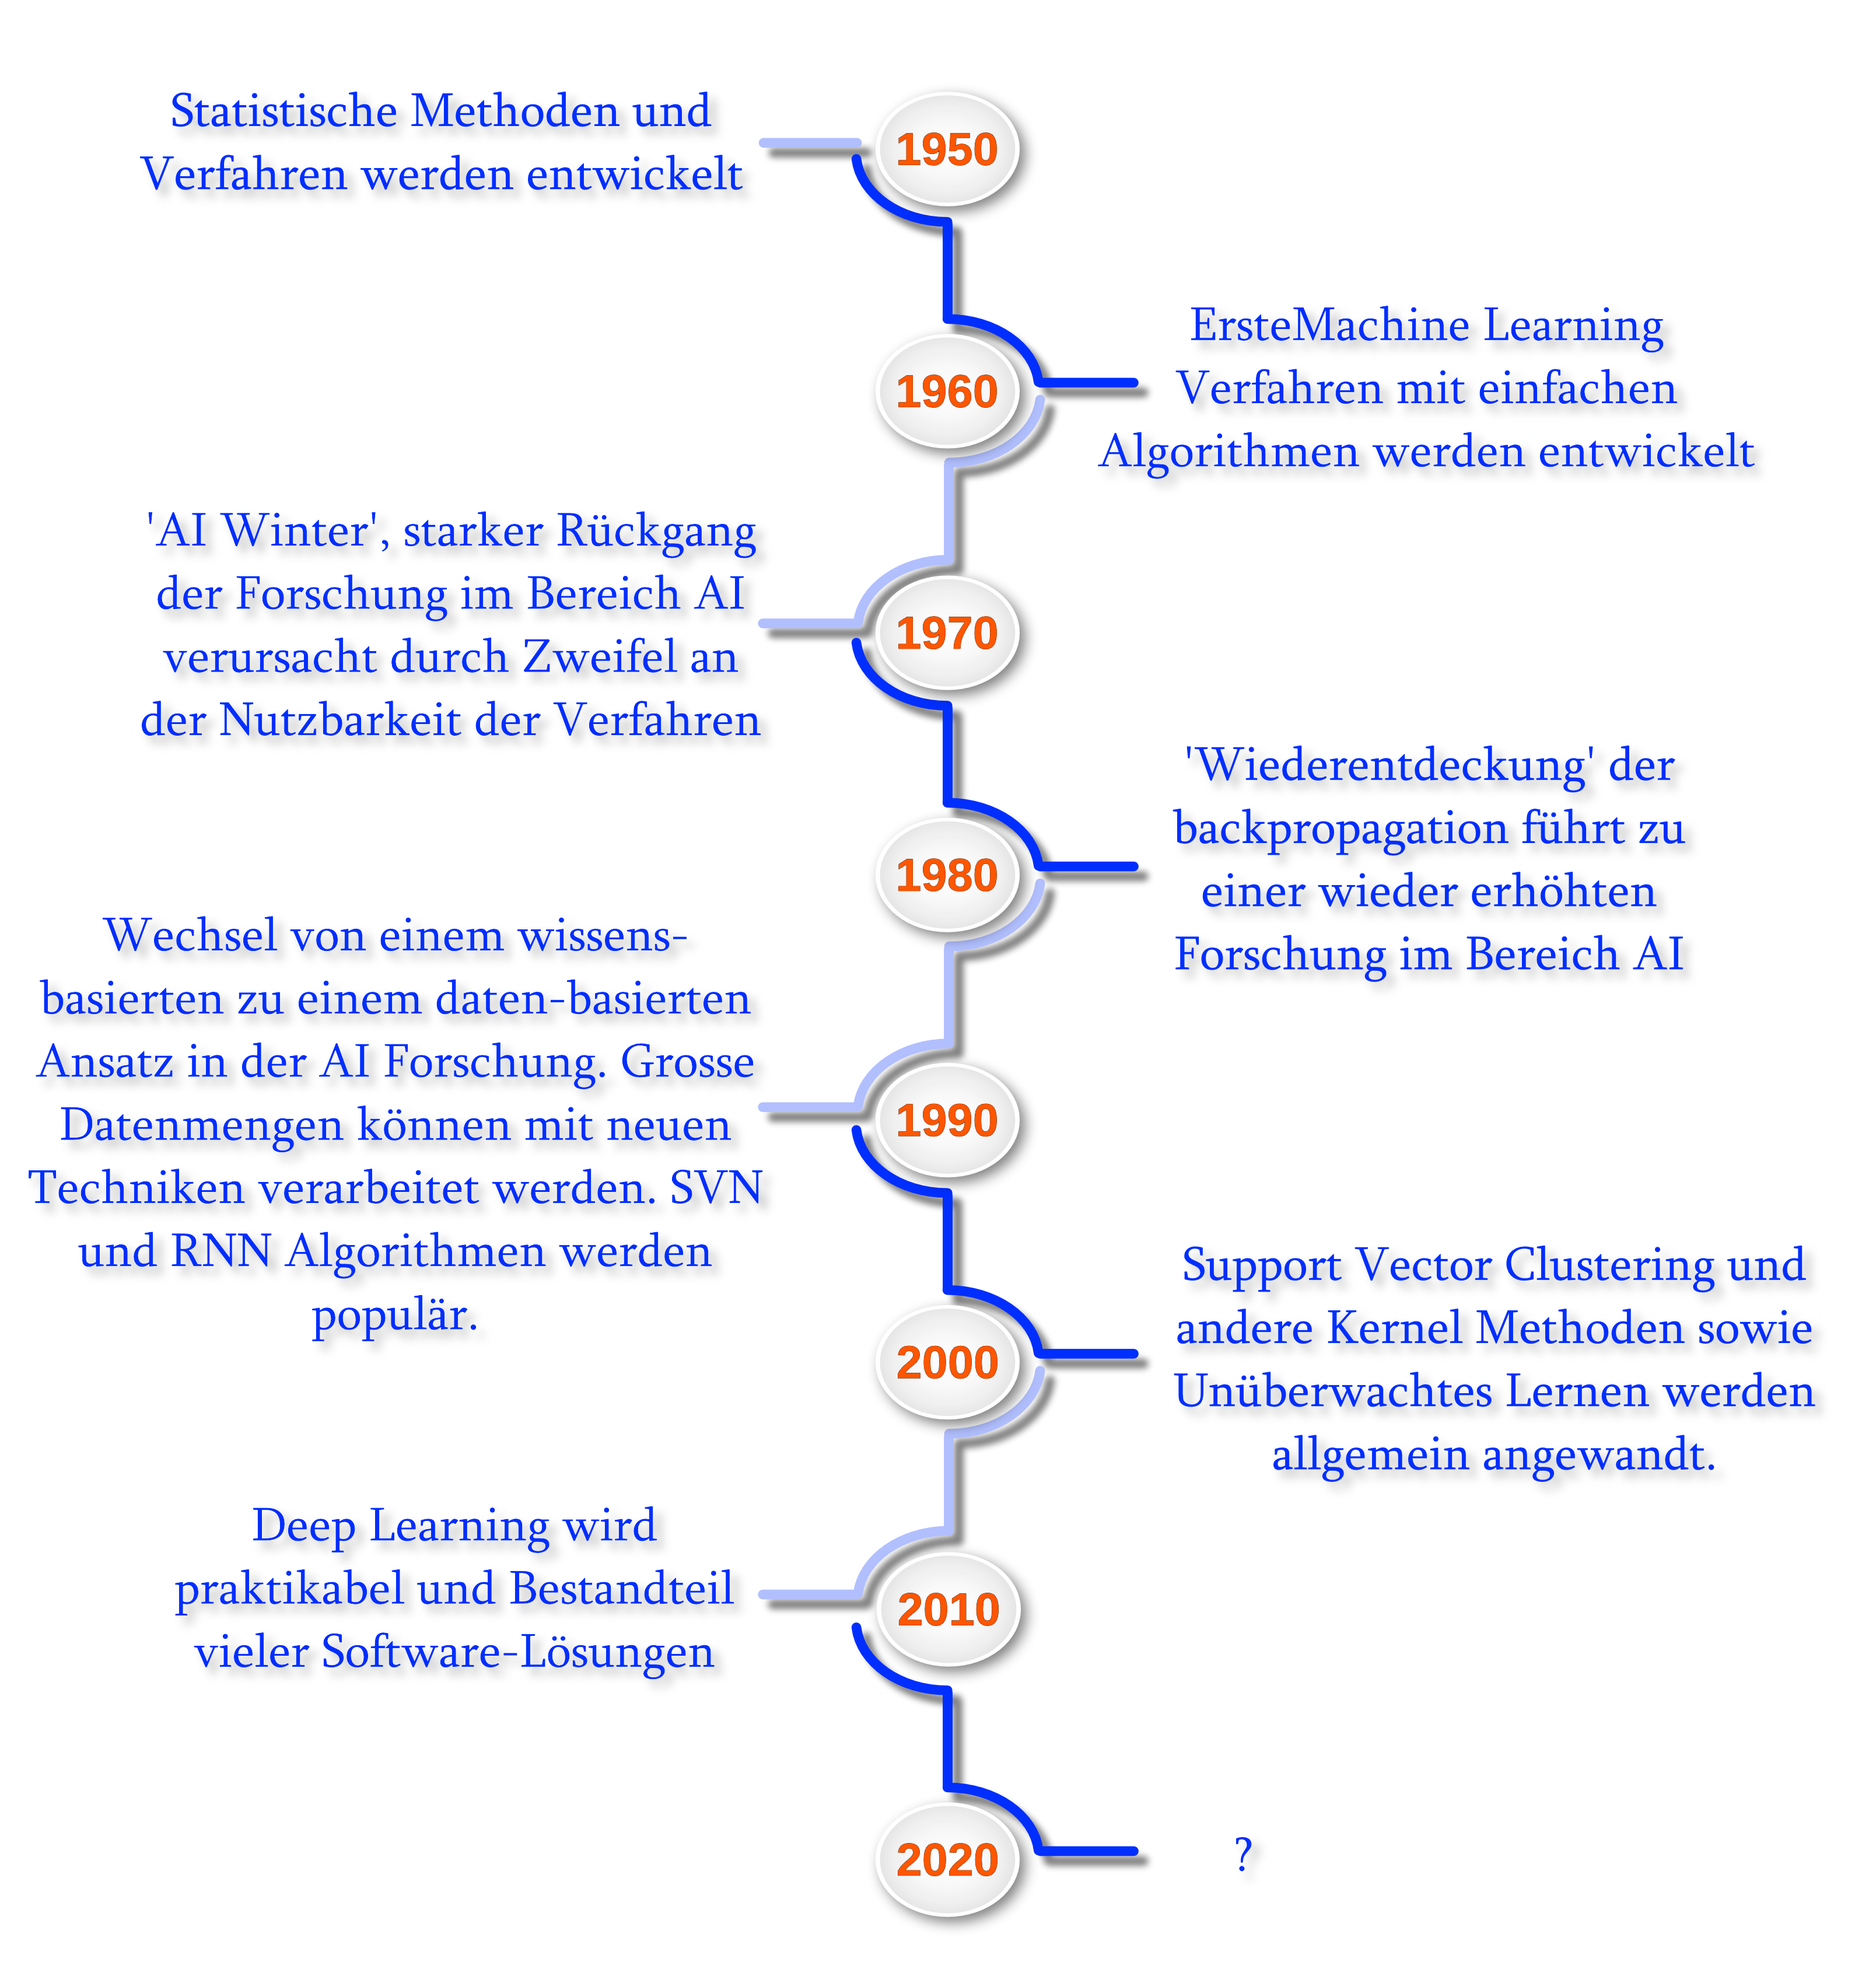
\includegraphics[width=\textwidth]{Bilder/ML-Timeline.png}
	\caption{Entwicklung des Machine Learning als Zeitachse.}
\end{figure}
\gls{ML} wird seit den 1960er Jahren angewendet, allerdings waren die erzielten Resultate lange Zeit für viele Anwendungen ungenügend. Durch die Verfügbarkeit von grossen Datenmengen (Big Data, Cloud) und der gesteigerten Rechenleistung der Rechner wurden nach der Jahrtausendwende so gute Fortschritte erzielt dass immer mehr Anwendungsmöglichkeiten für \gls{ML} Lösungen gefunden wurden. Während für viele Dienste im Internet (Bildersammlungen, Empfehlungssysteme) keine oder nur geringe Anforderungen an ein verständliches Modell gestellt werden gibt es einige Bereiche in denen besondere Regeln für die Nachvollziehbarkeit von Entscheidungen bestehen.

 Exemplarisch werden hier einige dieser Gebiete aufgeführt:

\begin{description}
  \item[Medizin] \gls{ML} Anwendungen für die Krebserkennung bieten grosses Potenzial. Insbesondere die ermüdenden Aufgabe auf Röntgen- oder MRT-Bildern Spuren eines Tumors zu erkennen könnten durch \gls{ML} abgelöst werden. Allerdings sind die Zulassungskriterien für solche Lösungen noch nicht definiert.
  \item[Justiz] Predictive Policing versucht mittels statistischer und \gls{ML} Verfahren Orte oder Personengruppen zu erkennen welche  Schauplatz oder Täter/Opfer eines Verbrechens werden könnten.
  \item[Selbstfahrende Fahrzeuge] Obwohl Selbstfahrende Fahrzeuge seit Jahren von allen grossen Fahrzeugherstellern entwickelt werden sind immer noch viele Fragen bezüglich der Haftung und Zulassung offen.
\end{description}

Aufgrund des Mangels an Techniken um fortgeschrittene \gls{ML} System zu Verstehen, entstand deshalb ein neues Forschungsgebiet \acrfull{xai} welches sich zum Ziel gesetzt hat Methoden und Werkzeuge zu entwickeln um \gls{ML} Modelle zu analysieren.

\chapter{Ein wager Begriff: Erklärbarkeit}
\section{Wie definiert sich Erklärbarkeit?}
\section{Unterschiedliche Ziele}
Eine Anwendung welche \acrfull{ML} einsetzt kann in mehrere Bereiche unterteilt werden.  Durch diese Aufteilung in verschiedene  Komponenten ergeben sich unterschiedliche Anforderungen an die Erklärbarkeit: \parencite{XAI2018}

\begin{description}
\item[Daten]
Aus der Sicht der Daten interessiert vor allem welcher Teil der Daten für das Ergebnis die Grösste Relevanz hat. Basierend auf dieser Erkenntnis kann das Datenset gezielt erweitert werden oder auch reduziert so dass ein ausgeglichenes Verhältnis erzeugt wird.

\item[Modell]
Kann man aus dem Modell Muster für eine bestimmte Kategorie ableiten? Dies kann helfen Fehlklassifizierungen von zusätzlichen Daten zu verhindern in dem überprüft wird ob das Modell die richtigen Features berücksichtigt.

\item[Vorhersage]
Erklärung weshalb ein bestimmtes Muster in den Daten zu der beobachteten Klassifizierung geführt hat. Dies ist insbesondere für Anwender/Kunden einer ML Lösung um a) das Verständnis für die Maschinelle Entscheidung zu erhöhen oder b) eine gesetzlich Vorgeschriebene Anfechtbarkeit der Entscheidung zu ermöglichen.
\end{description}

Ebenso gibt es bei den Interessengruppe unterschiedliche Anforderungen an die Erklärbarkeit einer ML Anwendung. Nach \parencite{Ras2018} werden dabei folgende Gruppierungen unterschieden:
\begin{description}
  \item[Experten]
  Diese Gruppe kann weiter unterteilt werden in
  	\begin{description}
  		\item[Forscher] Entwickelt neue Methoden und Algorithmen für das ML, verbessert bestehende Algorithmen
  		\item[Entwickler] Setzt bestehende Methodiken und Algorithmen ein um eine konkrete Aufgabenstellung zu lösen
	\end{description}
  \item[Benutzer]
  Auch bei den Benutzern gibt es verschiedene Ausprägungen
  	\begin{description}
  		\item[Eigentümer]
  		\item[Anwender]
  		\item[Person deren Daten verwendete wird]
  		\item[Anspruchsgruppe (Stakeholder)]
	\end{description}
\end{description}
Die Anforderungen an ein erklärbares Modell unterscheiden sich so stark je nach betrachtetet Komponente und der Anwendergruppe. Daraus ergibt sich dass verschiedene Techniken benötigt werden um AI Lösungen generell erklärbar zu machen.

\section{Herausforderungen durch Datenschutz}

\section{Diskriminierung}

\section{Bessere Anwendungen durch Einblick in die Funktionsweise}

\section{Weniger Angriffsflächen}

\section{Haftungsfragen}

\chapter{Anwendung von XAI auf Modelle}
Nach \parencite{Oh2019} hat Art des Modells von grossem Einfluss auf die Möglichkeiten der Erklärbarkeit. Generell wird unterschieden zwischen
\begin{description}
\item [Whitebox Modelle] sind unter der Kontrolle desjenigen welcher eine erklärende Analyse durchführt, sowohl die Daten wie der Aufbau des Modelles sind bekannt
\item[Blackbox Modelle] sind von unbekannter Struktur, der Anwender bekommt von einem gegebenen Input ein Resultat ohne den Ablauf der Entscheidungsfindung beobachten zu können
\end{description}

Aus der Vielzahl von Werkzeugen welche existieren um \acrfull{ML} Modelle zu analysieren gilt es die für den jeweiligen Use Case relevanten Werkzeuge anzuwenden.
TODO: Übersicht der Techniken und Anwendungsbereiche wie in der Grafik

\section{Use Cases}
\subsection{Exploration}
\subsection{Feature Engineering}
\subsection{Modelle erstellen}
\subsection{Modelle interpretieren}

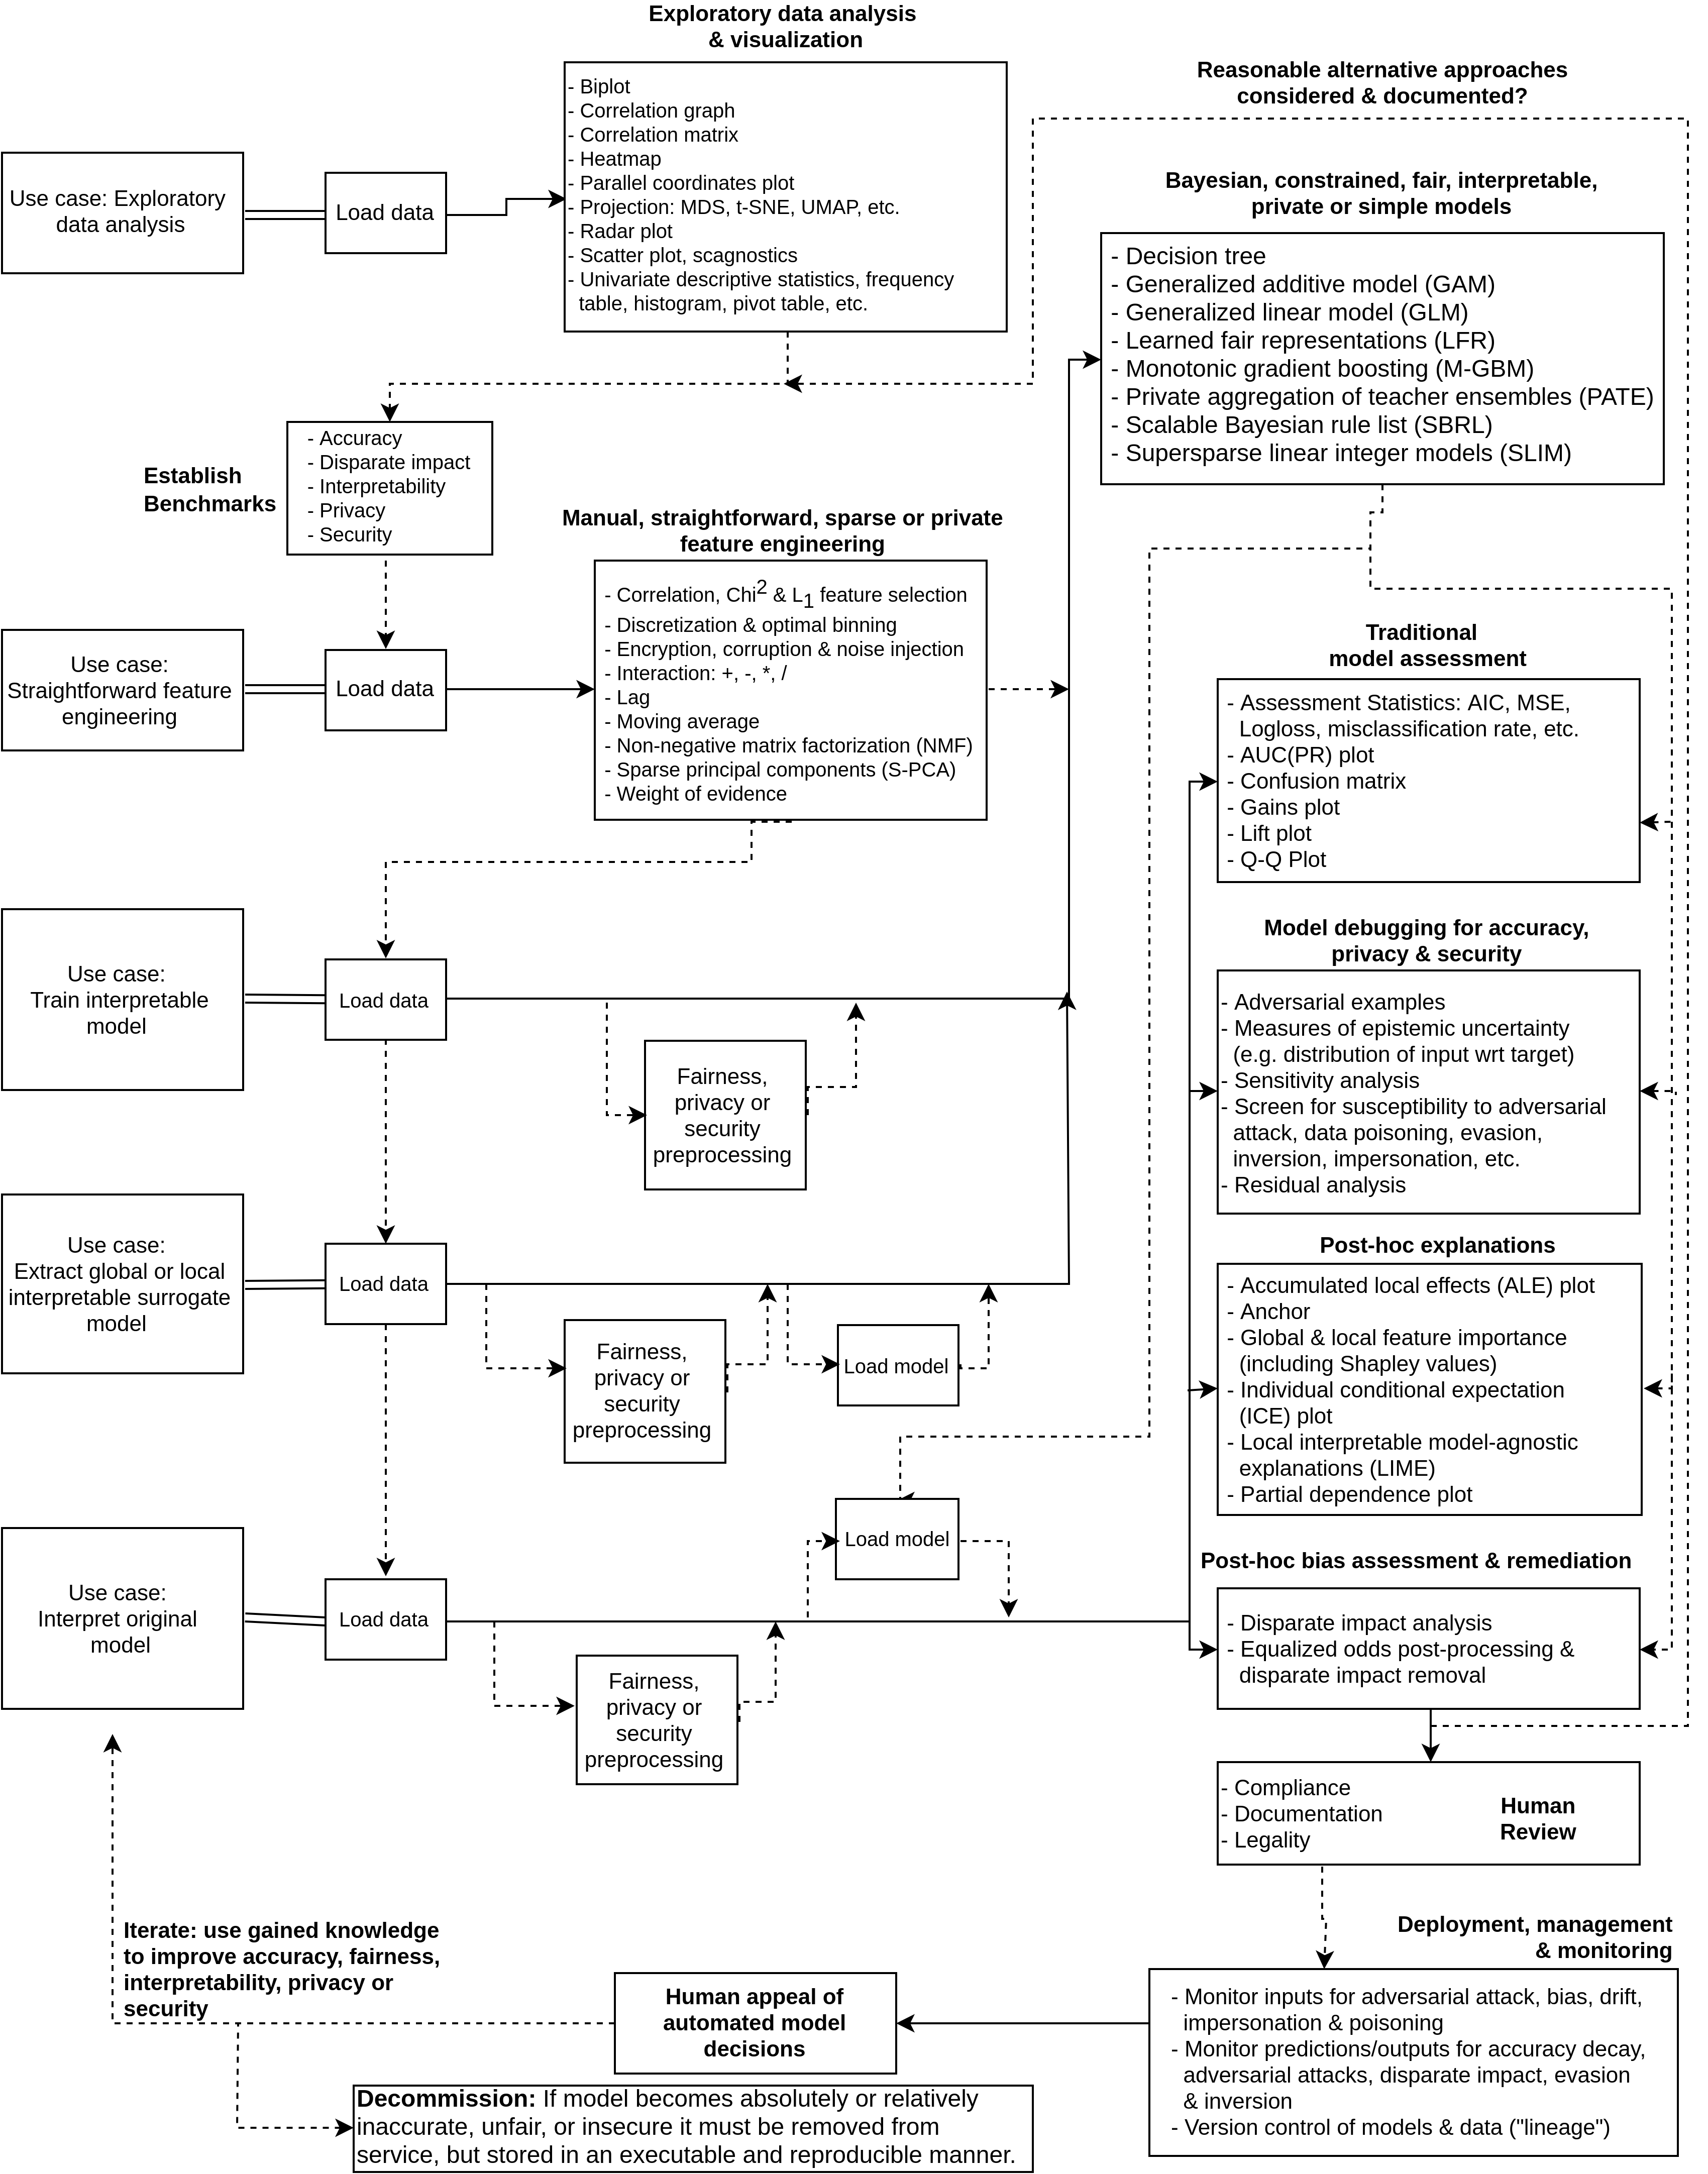
\includegraphics[width=\textwidth]{Bilder/blueprint.png}
\captionof{figure}{Quelle: https://github.com/h2oai/mli-resources}

\section{Grundsätzlich erklärbare Algorithmen}
\subsection{Lineare Regression}
\subsection{Entscheidungsbäume}
Entscheidungsbäume (engl. Decision Tree) können bei einer geringen Anzahl von Parametern gut visualisiert werden.
\begin{center}
\begin{minipage}[t]{0.45\linewidth}
Die Regeln nach denen sich ein \Gls{DT} aufteilt können als Text dargestellt werden. Intuitiv besser verständlich sind jedoch grafische Darstellungen welche entweder den Baum als Struktur oder in einem Diagramm als Fläche darstellen.
\end{minipage}\hfill
\begin{minipage}[t]{0.45\linewidth}
\begin{lstlisting}
|--- petal width (cm) <= 0.80
|   |--- class: 0
|--- petal width (cm) >  0.80
|   |--- petal width (cm) <= 1.75
|   |   |--- class: 1
|   |--- petal width (cm) >  1.75
|   |   |--- class: 2
\end{lstlisting}
\end{minipage}
\end{center}

\begin{center}
\begin{minipage}[t]{0.45\linewidth}
\centering
	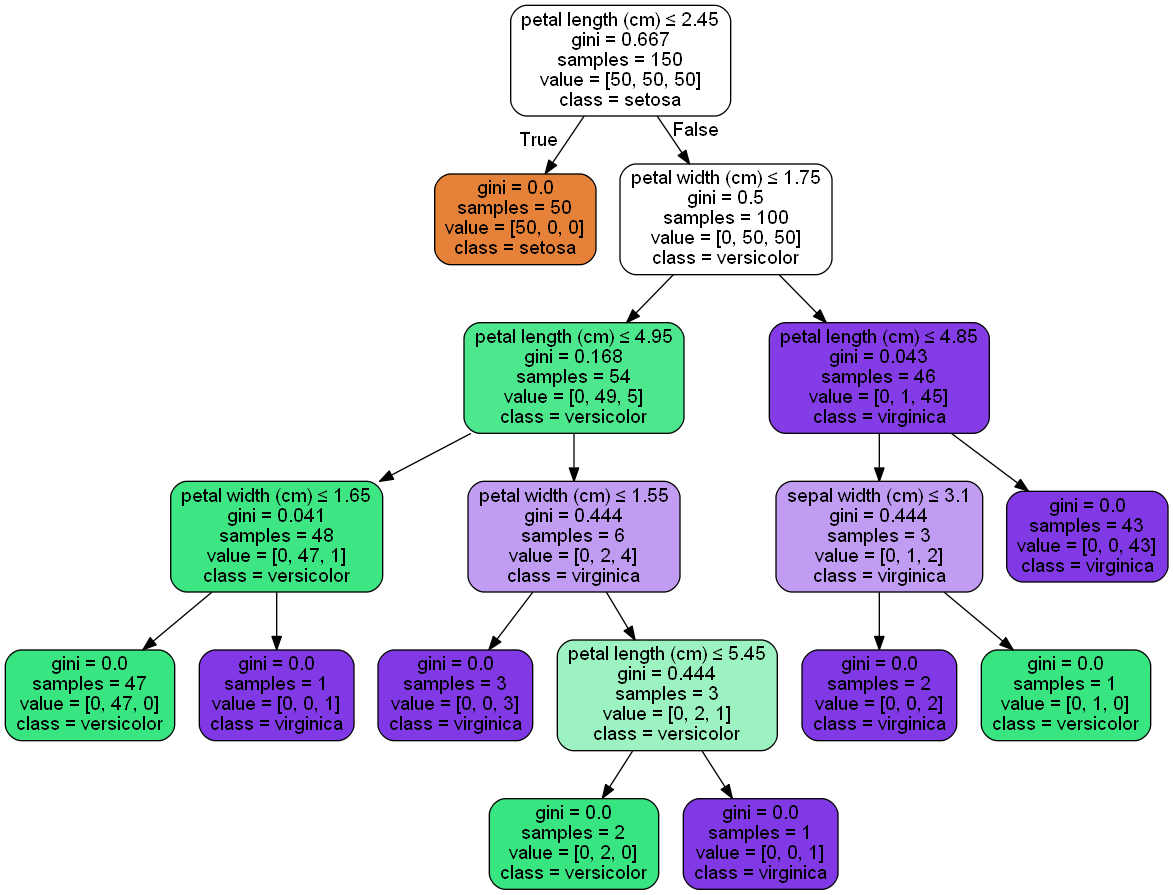
\includegraphics[width=\textwidth]{Bilder/iris-dt-explained.png}
	 \captionof{figure}{Entscheidungsbaum visualisiert.}
\end{minipage}\hfill
\begin{minipage}[t]{0.45\linewidth}
\centering
	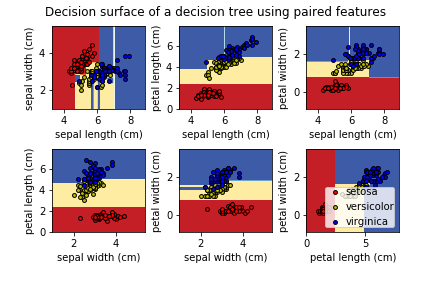
\includegraphics[width=\textwidth]{Bilder/iris-dt-decision-surface.png}
	 \captionof{figure}{Entschdeidungsbaum als Flächen dargestellt}
\end{minipage}
\end{center}
Source Code \ref{dt-vis} (benötigt min. scikit-learn 0.22)

\subsection{GLM/GAM}
\subsection{RuleFit}
\subsection{Naive Bayes}

\section{Bilderkennung}
In den letzten Jahrzehnten wurden grosse Fortschritte in der Bilderkennung gemacht. Verantwortlich dafür sind vor allem Neuronale Netze, insbesondere die Techniken \acrfull{cnn} in Zusammenhang mit {dnn}. Neuronale Netze, insbesondere die für Bilderkennung weit verbreiteten \acrfull{dnn}, sind ohne weitere Hilfsmittel kaum zu analysieren.
Durch den starken Fokus auf Neuronale Netze bei der Bilderkennung sind für diese Technik auch einige Methoden vorhanden um das Verhalten eines Modelles  auf ein Bild darzustellen.
\subsection{Analyse Neuronaler Netze}
\subsubsection*{Eigenes Modell}
\imgText{dog-good-heatmap.png}{ 
Ein präzises Model verwendet keine Bildpunkte welche nicht dem gesuchten Objekt zugehören.
}

\imgText{dog-bad-heatmap.png}{ 
Obwohl in diesem Beispiel das Objekt korrekt erkannt wurde ist die präzision des Models klein.
}

\imgText{cat-good-heatmap.png}{ 
Allerdings ist auch eine gute Übereinstimmung mit dem Objekt keine Garantie dass die richtige Klasse gefunden wird.
}

\imgText{cat-bad-heatmap.png}{ 

}
\subsubsection*{ImageNet Modell}
Das für die folgenden Analysen verwendete Modell \parencite{Simonyan2014} stammt aus der ImageNet Challenge \cite{imageNet} aus dem Jahr 2014 und ist frei verfügbar. ImageNet definiert 1001 Klassen von Objekten welche erkannt werden. Eine Klassifikation mit \cite{TensorFlow} erzeugt eine Liste mit den Wahrscheinlichkeiten für alle Klassen. Mit den \acrfull{XAI} Techniken kann für jede Klasse visualisiert werden welche Bildbereiche für diese Klassifikation relevant sind.

Mittels dem Modell VGG16 aus der Tensorflow Bibliothek \cite{vgg16} wurde folgendes Bild analysiert:
\imgText{Mira.jpg}{
		\begin{tabular}{ |c|c| } 
		 \hline
		 Klasse & Wahrscheinlichkeit \\
		 \hline
		 Egyptian cat1 & 55.31\% \\ 
		 tabby & 8.59\% \\ 
		 tiger cat & 5.59\% \\ 
		 carton & 4.63\% \\
		 toilet tissue & 3.55\% \\
		 \hline
		\end{tabular}
		\break
		Während die ersten drei Klassen alle eine Katzenart definieren ist die vierte Klasse ``Karton'' und die Fünfte ``Toilettenpapier'' unpassend. An und für sich ist die Wahrscheinlichkeit für ``toilet tissue'' mit 3.55\% sehr klein, dennoch stellt sich die Frage weshalb dies die gegenüber den verschiedenen Katzenarten nächste Klasse ist.
}

\subsubsection*{Grad CAM} \break
\Gls{Grad CAM} ist eine Technik \parencite{Selvaraju2016} um auf der Basis von Gradienten die für eine Bildklassifikation relevanten Bereiche eines Bildes hervorzuheben. Während die relevantesten Bereiche (gelb gefärbt) um den Kopf und vor allem den Ohren der Katze sind, zeigen die Darstellungen für die unpassenden Klassen auf Bereiche des Bodens.
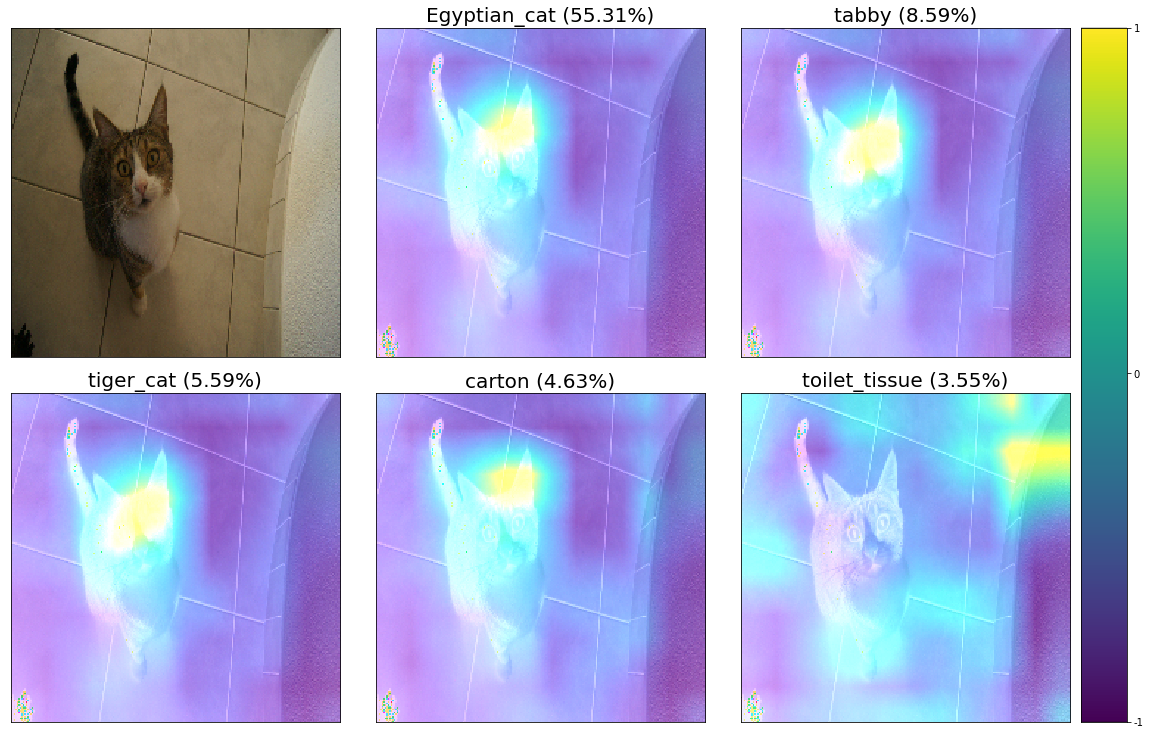
\includegraphics[width=\textwidth]{Bilder/Grad-Cam-Classes.png}

\subsubsection*{Occlusion Sensitivity} \break
Eine weitere Variante um relevante Bildbereiche aufzudecken ist Occlusion Sensitivity. Mit diesem Verfahren tritt deutlicher als bei Grad CAM die Fokusierung auf den Boden bei den beiden Falschen Klassifizierungen zutage.
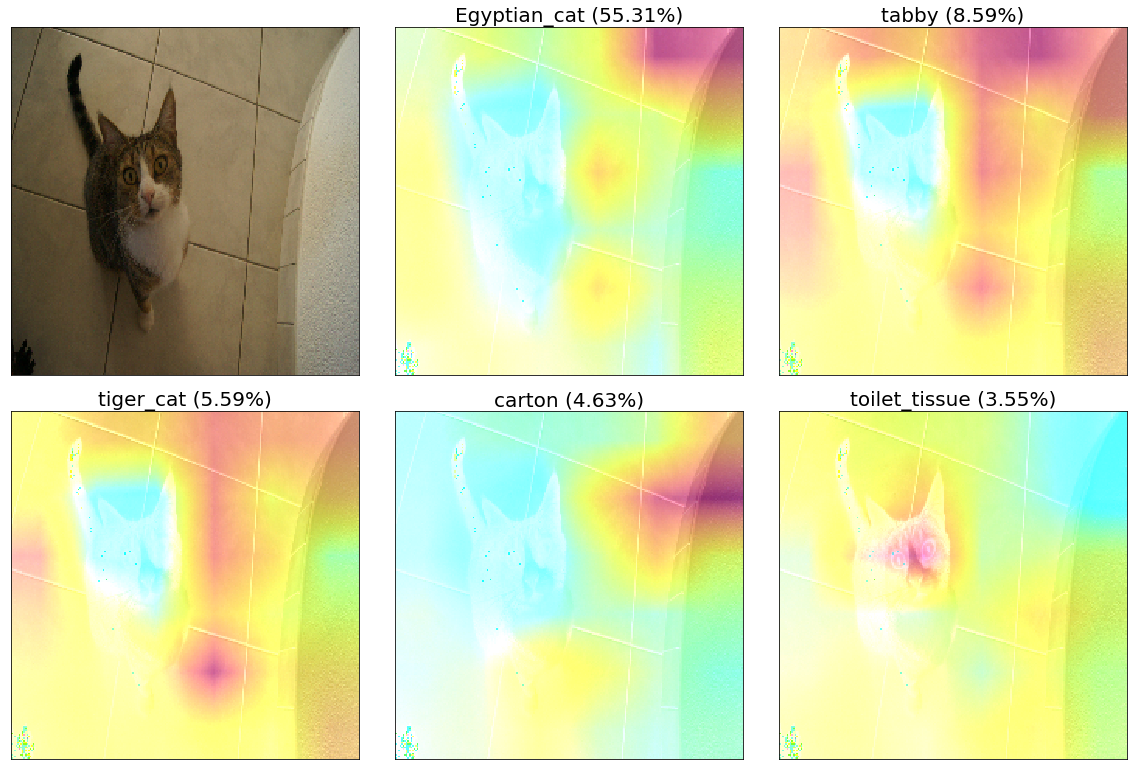
\includegraphics[width=\textwidth]{Bilder/OcclusionSensitivity-Classes.png}

\subsubsection*{LRP}
\acrfull{lrp} ist eine Technik welche ebenfalls versucht die Vorhersage eines Klassifizierers zu erklären. 

\url{ttps://github.com/VigneshSrinivasan10/interprettensor}
\url{https://github.com/sebastian-lapuschkin/lrp_toolbox}

\subsubsection*{Lime}
\url{https://arxiv.org/abs/1602.04938}
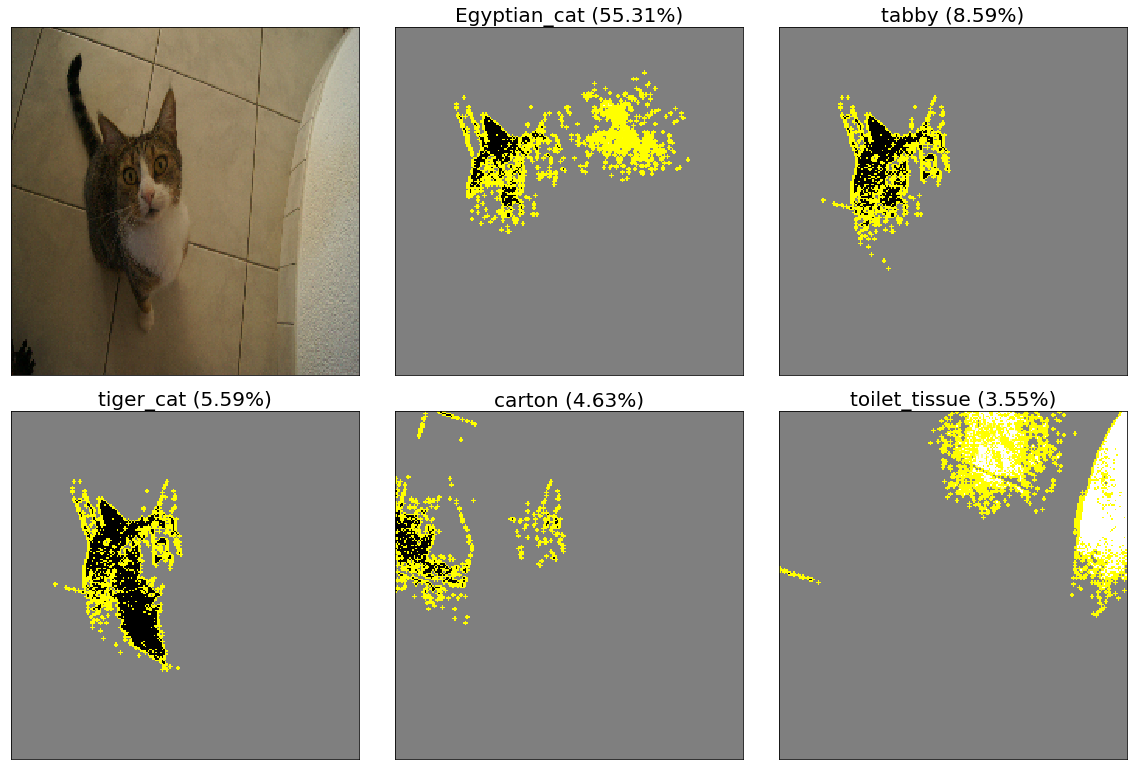
\includegraphics[width=\textwidth]{Bilder/Lime-Classes.png}

\subsubsection*{TCAV}
\url{https://github.com/tensorflow/tcav}

\subsubsection*{SVCCA}
\url{https://ai.googleblog.com/2017/11/interpreting-deep-neural-networks-with.html}

\section{Texterkennung}
\url{https://eli5.readthedocs.io/en/latest/tutorials/sklearn-text.html}

\chapter{Schwächen von ML Modellen erkennen}
\section{Diskriminierung durch Bias}
\section{Adversarial Attacks}
\section{Data Poisoning}

\chapter{Weiterentwicklung von XAI}

\chapter{Anhang}
\section{Source Code}
\label{dt-vis}

\subsection{Entscheidungsbaum Visualisierung mit sklearn und Graphviz}
\begin{lstlisting}[language=Python, caption=Decision Tree Visualisierung]
from sklearn.datasets import load_iris
from sklearn import tree
from sklearn import datasets

X, y = load_iris(return_X_y=True)
clf = tree.DecisionTreeClassifier()
clf = clf.fit(X, y)

iris = datasets.load_iris()

dot_data = tree.export_graphviz(clf, out_file=None, 
                      feature_names=iris.feature_names,  
                      class_names=iris.target_names,  
                      filled=True, rounded=True,  
                      special_characters=True)  

# print tree as text
from sklearn.tree import export_text
r = export_text(clf, feature_names=iris['feature_names'])
print(r)

# print tree as colored top-down tree
import graphviz
graph = graphviz.Source(dot_data)  
graph 

# plot decision surface
import numpy as np
import matplotlib.pyplot as plt
# Parameters
n_classes = 3
plot_colors = "ryb"
plot_step = 0.02

for pairidx, pair in enumerate([[0, 1], [0, 2], [0, 3],
                                [1, 2], [1, 3], [2, 3]]):
    # We only take the two corresponding features
    X = iris.data[:, pair]
    y = iris.target
    
    # Train
    dTree = tree.DecisionTreeClassifier().fit(X, y)

    # Plot the decision boundary
    plt.subplot(2, 3, pairidx + 1)

    x_min, x_max = X[:, 0].min() - 1, X[:, 0].max() + 1
    y_min, y_max = X[:, 1].min() - 1, X[:, 1].max() + 1
    xx, yy = np.meshgrid(np.arange(x_min, x_max, plot_step),
                         np.arange(y_min, y_max, plot_step))
    plt.tight_layout(h_pad=0.5, w_pad=0.5, pad=2.5)

    Z = dTree.predict(np.c_[xx.ravel(), yy.ravel()])
    Z = Z.reshape(xx.shape)
    cs = plt.contourf(xx, yy, Z, cmap=plt.cm.RdYlBu)

    plt.xlabel(iris.feature_names[pair[0]])
    plt.ylabel(iris.feature_names[pair[1]])

    # Plot the training points
    for i, color in zip(range(n_classes), plot_colors):
        idx = np.where(y == i)
        plt.scatter(X[idx, 0], X[idx, 1], c=color, label=iris.target_names[i],
                    cmap=plt.cm.RdYlBu, edgecolor='black', s=15)

plt.suptitle("Decision surface of a decision tree using paired features")
plt.legend(loc='lower right', borderpad=0, handletextpad=0)
plt.axis("tight")
\end{lstlisting}
https://scikit-learn.org/stable/modules/tree.html

\subsection{Bild-Klassifikation mit tf-explain}
Das folgende Programm erzeugt mit den Bibliotheken Tensorflow (2.0) und tf-explain und en Algorithmen ``Grad CAM'' und ``Integrated Gradients'' Visualisierungen einer Bild-Klassifizierung. 
\begin{lstlisting}[language=Python, caption=Visualisiertes Neuronales Netz mit Tensorflow und tf-explain]
import tensorflow as tf
from keras.applications.vgg16 import VGG16
from keras.preprocessing.image import load_img
from keras.preprocessing.image import img_to_array
from keras.applications.vgg16 import preprocess_input
from keras.applications.vgg16 import decode_predictions

model = tf.keras.applications.vgg16.VGG16(weights="imagenet", include_top=True)

#print(model.summary())

imageOrig = load_img('D:/Master Thesis/dogs-vs-cats/test/DSC05797.JPG', target_size=(224, 224))
imageArr = img_to_array(imageOrig)  #output Numpy-array

imageReshaped = imageArr.reshape((1, imageArr.shape[0], imageArr.shape[1], imageArr.shape[2]))

image = preprocess_input(imageReshaped)
predictions = model.predict(imageReshaped)

import numpy as np
top5predictions = np.argsort(predictions)[0,::-1][:5]

labels = decode_predictions(predictions)

for label in labels[0]:
    print('%s (%.2f%%)' % (label[1], label[2]*100))
    
from tf_explain.core.grad_cam import GradCAM
from mpl_toolkits.axes_grid1 import ImageGrid

def createImageGrid(imageOrig, predictions, labels, explainer, explainerArgs):
    camImages = [imageOrig]
    fig = plt.figure(figsize=(20., 20.))
    grid = ImageGrid(fig, 111,  # similar to subplot(111)
                 nrows_ncols=(2, 3),
                 axes_pad=0.5,  # pad between axes in inch.
                 )
    for class_index in top5predictions:
        camImages.append(explainer.explain(class_index=class_index, **explainerArgs))
    
    i = -1
    for ax, im in zip(grid, camImages):
        # Iterating over the grid returns the Axes.
        ax.set_xticks([])
        ax.set_yticks([])
        label = labels[0][i]
        if i >= 0:
            ax.set_title('%s (%.2f%%)' % (label[1], label[2]*100), fontsize=20)
        ax.imshow(im)
        i = i + 1

    plt.show()


explainer = GradCAM()
createImageGrid(imageOrig, predictions, labels, explainer, {'model': model, 'layer_name': 'block5_conv3', 'validation_data': data})

from tf_explain.core.gradients_inputs import GradientsInputs
explainer = GradientsInputs()
createImageGrid(imageOrig, predictions, labels, explainer, {'model': model, 'validation_data': (np.array([imageArr]), None)})

from tf_explain.core.integrated_gradients import IntegratedGradients

explainer = IntegratedGradients()
createImageGrid(imageOrig, predictions, labels, explainer, {'model': model, 'validation_data': (np.array([imageArr]), None)})
\end{lstlisting}
https://github.com/sicara/tf-explain

\subsection{Visualisierung einer Klassifikation mit lime}
\url{https://github.com/marcotcr/lime/blob/master/doc/notebooks/Tutorial\%20-\%20Image\%20Classification\%20Keras.ipynb}
\begin{lstlisting}[language=Python, caption=Visualisiertes Neuronales Netz mit Tensorflow und lime]
import lime 
from lime import lime_image

explainer = lime_image.LimeImageExplainer()


explanation = explainer.explain_instance(np.vstack([imageArr]), model.predict, top_labels=5, hide_color=0, num_samples=1000)

from skimage.segmentation import mark_boundaries

camImages = [imageOrig]
fig = plt.figure(figsize=(20., 20.))
grid = ImageGrid(fig, 111,  # similar to subplot(111)
             nrows_ncols=(2, 3),
             axes_pad=0.5,  # pad between axes in inch.
             )
for class_index in range(0,5):
    temp, mask = explanation.get_image_and_mask(explanation.top_labels[class_index], positive_only=True, num_features=5, hide_rest=True)
    camImages.append(mark_boundaries(temp / 2 + 0.5, mask))

i = -1
for ax, im in zip(grid, camImages):
    # Iterating over the grid returns the Axes.
    ax.set_xticks([])
    ax.set_yticks([])
    label = labels[0][i]
    if i >= 0:
        ax.set_title('%s (%.2f%%)' % (label[1], label[2]*100))
    ax.imshow(im)
    i = i + 1

plt.show()
\end{lstlisting}
\appendix
% List of Figures
\listoffigures
% List of Tables
\begingroup
\let\clearpage\relax
\listoftables
% Glossary
\printglossary[type=\acronymtype]
\printglossary[type=main]
% Bibliography
\printbibliography

\renewcommand\bibname{Linkverzeichnis}
\begin{thebibliography}{99}\label{links}
   \bibitem{vgg16} VGG16: Modell für Imagenet Klassifikationen \break \url{https://github.com/tensorflow/tensorflow/blob/r1.8/tensorflow/python/keras/_impl/keras/applications/vgg16.py}
   \bibitem{imageNet} ImageNet Challenge \break \url{http://www.image-net.org/challenges/LSVRC/}
   \bibitem{iML}Interpretable Machine Learning, A Guide for Making Black Box Models Explainable \break \url{https://christophm.github.io/interpretable-ml-book/rulefit.html}
\end{thebibliography}
%Index
\addcontentsline{toc}{chapter}{Index}
%\printindex
% Appendices
\lstlistoflistings
\endgroup

\end{document}
